\documentclass[10pt]{ctexart}
\usepackage{amsmath,amsfonts,amssymb,amsthm}
\usepackage[a4paper,left=2.5cm,right=2.5cm,top=2cm,bottom=2cm]{geometry}
\usepackage{graphicx,booktabs}
\usepackage{float,bm}
\usepackage{subfigure}
\author{2000012425 张弛}
\title{计算物理第六次作业}
\CTEXsetup[format={\Large\bfseries}]{section}
\newtheorem*{answer}{答}
\newtheorem*{solution}{解}
\newtheorem*{fuck}{证明}
\begin{document}
\maketitle
1.选取某种程序自带的随机数产生方法,产生一组$[0-1]$之间均匀分布的随机数.

1.1

利用随机数,编写程序对下列积分进行蒙特卡洛计算。重复上述步骤多次(如:1000次),给出积分值的分布曲线,讨论该分布与撒点数的关系。
$$\int_{0}^{1}dx\ exp[-100\times(x-0.5)^2].$$
\begin{solution}
    分别设撒点数为$10^2,10^3,10^4$。分别计算积分$1000$次,并画出积分值的分布曲线。

    借助程序"HW6计物第一题撒点法.py"得到下图
    \begin{figure}[H]
        \centering
        \begin{minipage}{0.45\linewidth}
            \centering
            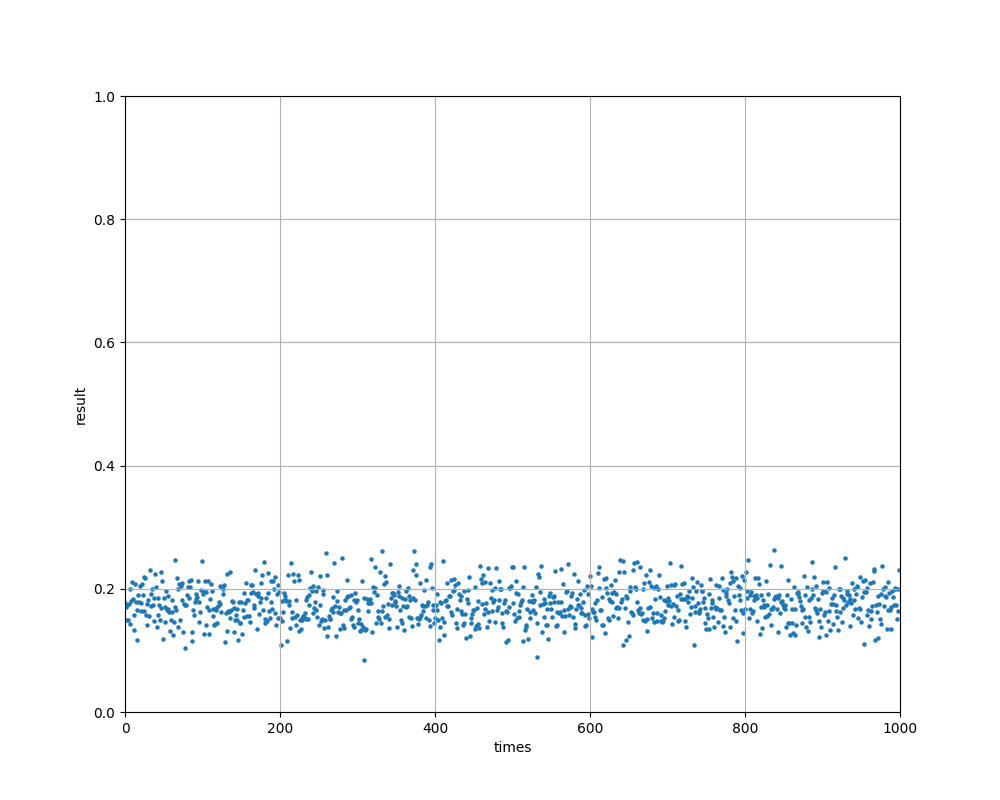
\includegraphics[width=7cm]{sprinkle_100.png}
            \caption{$10^2$次撒点}
        \end{minipage}
        \qquad
        \begin{minipage}{0.45\linewidth}
            \centering
            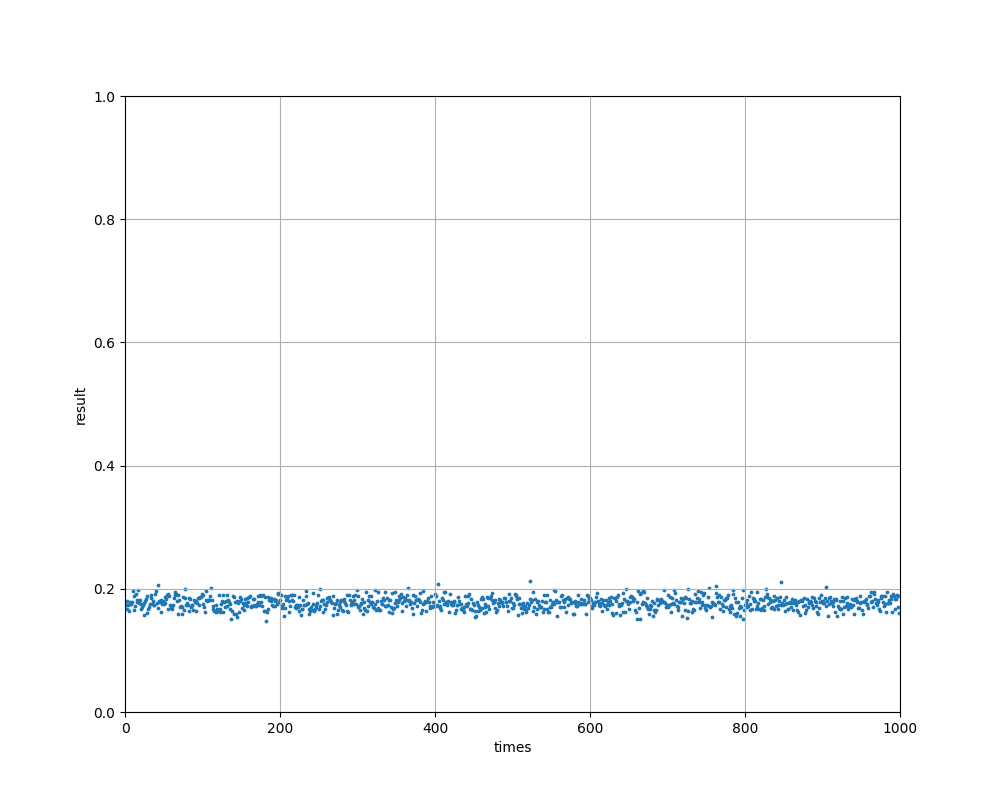
\includegraphics[width=7cm]{sprinkle_1000.png}
            \caption{$10^3$次撒点}
        \end{minipage}
    \end{figure}
    \begin{figure}[H]
        \centering
        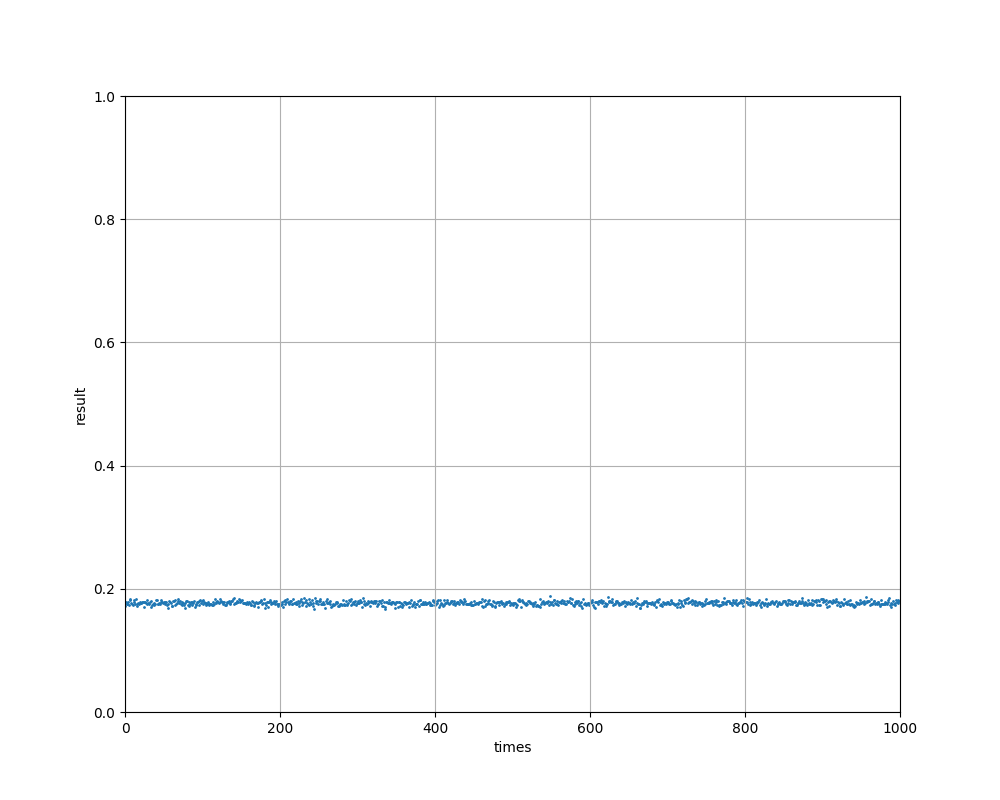
\includegraphics[width=9cm]{sprinkle_10000.png}
        \caption{$10^4$次撒点}
    \end{figure}
    可以看出计算结果集中在精确值0.177附近,且撒点数越多,方差越小。
\end{solution}
1.2

利用随机数,编写程序对下列多维积分进行蒙特卡洛估算:
$$\int_{0}^{1}\cdots\int_{0}^{1}dx_1\cdots dx_9\ exp\left [-100\times\sum\limits_{i=1}^{i=9}(x_i-0.5)^2\right ].$$
\begin{solution}
    依然使用撒点法。在九维空间中撒点$10^7$次,取函数值的平均值。借助程序"HW6计物第一题多维积分.py"得到10000次计算结果分布如下
    \begin{figure}[H]
        \centering
        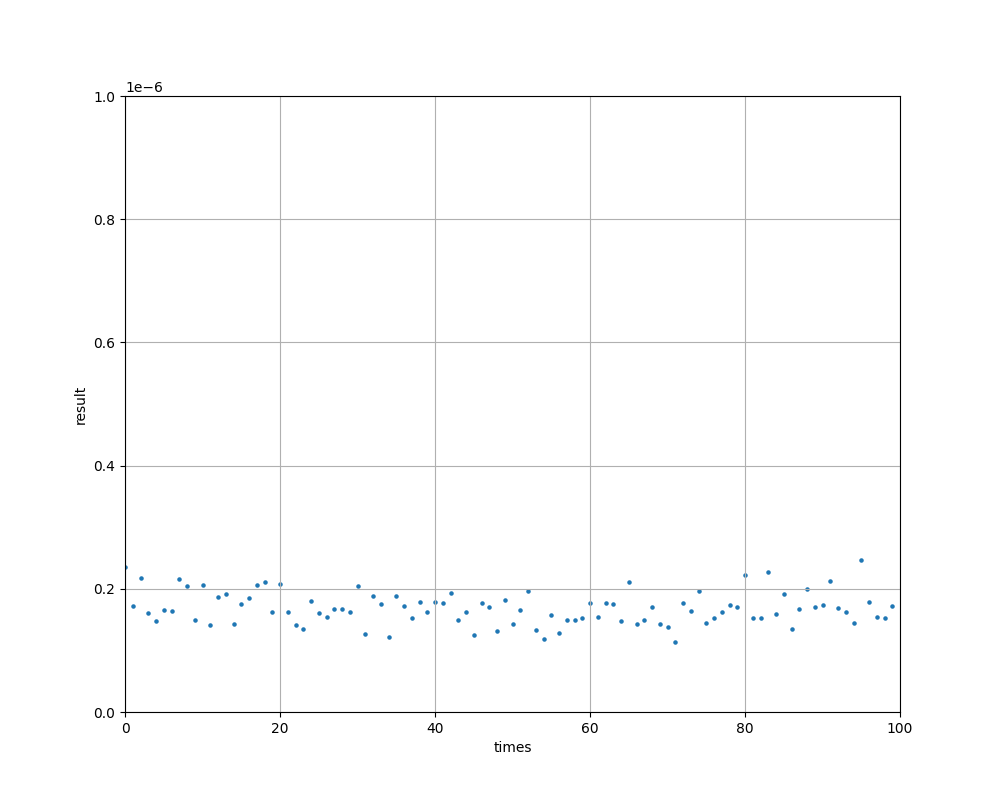
\includegraphics[width=10cm]{HIghD_10000000.png}
        \caption{$10^7$次撒点}
    \end{figure}
结果基本集中在精确值$1.7\times 10^{-7}$附近。结果可信。
\end{solution}
2.1

题目不抄了。
\begin{solution}
    蒙卡的基本思路是,对于一个给定的态,按顺序随机改变自旋的值,计算改变前后的能量差值$\Delta E$,这样考虑可以提高计算效率。若
    $$\Delta E<0,$$
    则接受这个改变。若
    $$\Delta E>0,$$
    则按照概率
    $$e^{-\Delta E/kT}$$
    接受改变。每一次概率选择结束计算能量(加上$\Delta E$),所有的结果求和取平均得到平均能量$E$。画出不同温度$T$下的能量$E$,用差分来近似
    温度$T$下的热容$C$。

    若要计算磁化率,则在计算$\Delta E$时,加入外场与自旋磁矩的相互作用项$CS$,在多轮次蒙卡循环中计算磁化强度$M$平均值即可。

    晶格结构是循环周期的。

    不妨$J=1,C=-1,k=1$。

    先进行一些粗略计算,仅看热容$C$的温度$T$依赖。蒙卡循环$10^3$次。温度$T$范围$0.5-9.5K$。借助程序“HW6计物第二题热容试探.py”,对于$10\times 10$格子有
    \begin{figure}[H]
        \centering
        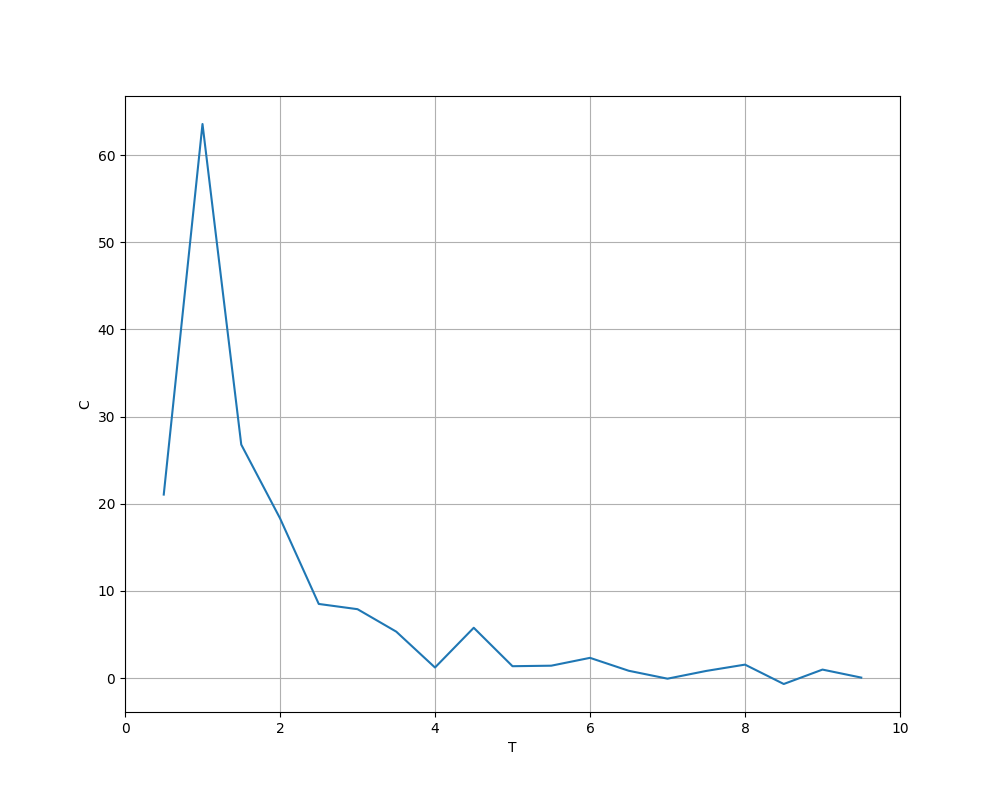
\includegraphics[width=10cm]{Rough_10.png}
        \caption{$10\times 10$热容$C$的温度$T$依赖粗略计算}
    \end{figure}
    以及对$40\times 40$和$80\times 80$格子有
    \begin{figure}[H]
        \centering
        \begin{minipage}{0.45\linewidth}
            \centering
            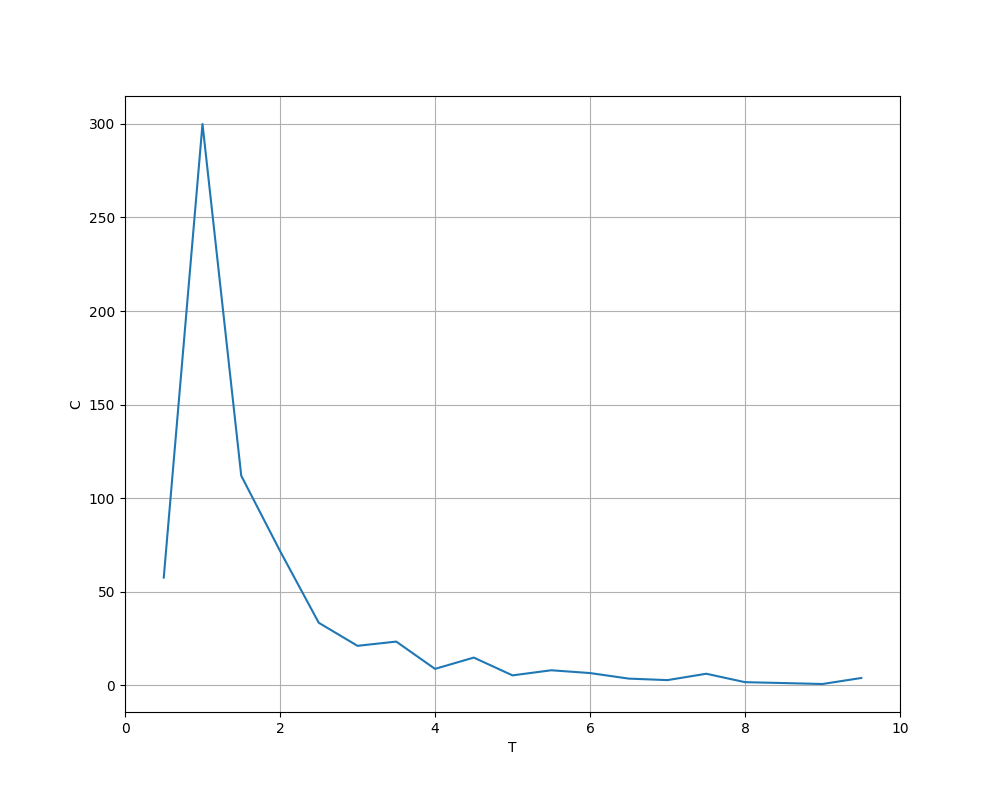
\includegraphics[width=8cm]{Rough_40.png}
            \caption{$40\times 40$热容$C$的温度$T$依赖粗略计算}
        \end{minipage}
        \qquad
        \begin{minipage}{0.45\linewidth}
            \centering
            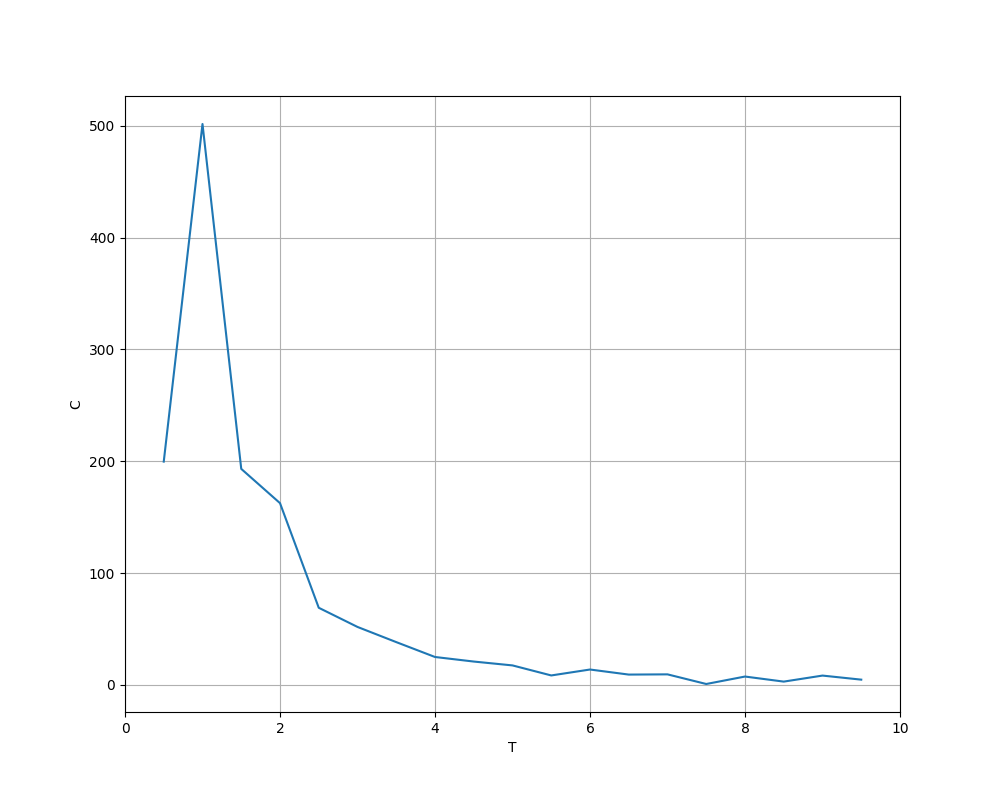
\includegraphics[width=8cm]{Rough_80.png}
            \caption{$80\times 80$热容$C$的温度$T$依赖粗略计算}
        \end{minipage}
    \end{figure}
    看到相变在$0.5-1.5K$之间。下面正式计算能量$E$,热容$C$与磁化率$\chi$的在相变温度附近的温度$T$依赖。蒙卡循环$10^5$次。温度$T$范围$0.6-1.5K$。借助程序“HW6计物第二题能量.py”“HW6计物第二题热容.py”和
    “HW6计物第二题磁化率.py”得到下面结果。对于$10\times 10$格子,能量有
    \begin{figure}[H]
        \centering
        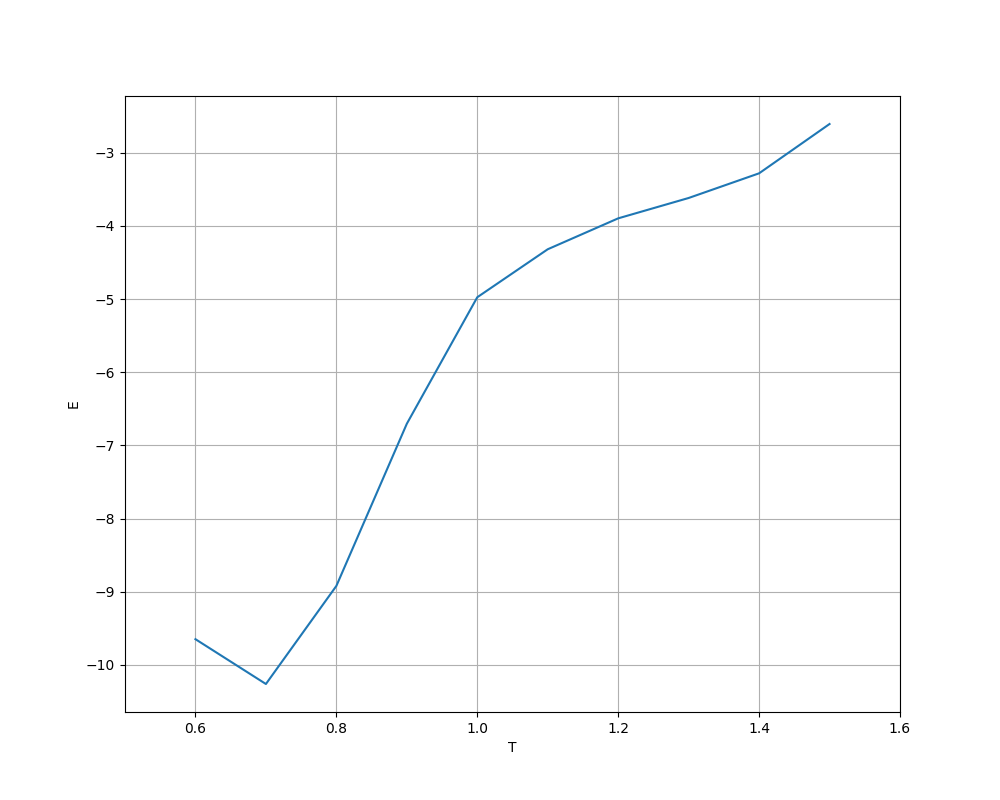
\includegraphics[width=10cm]{E_10.png}
        \caption{$10\times 10$能量$E$的温度$T$依赖}
    \end{figure}
    热容和磁化率有
    \begin{figure}[H]
        \centering
        \begin{minipage}{0.45\linewidth}
            \centering
            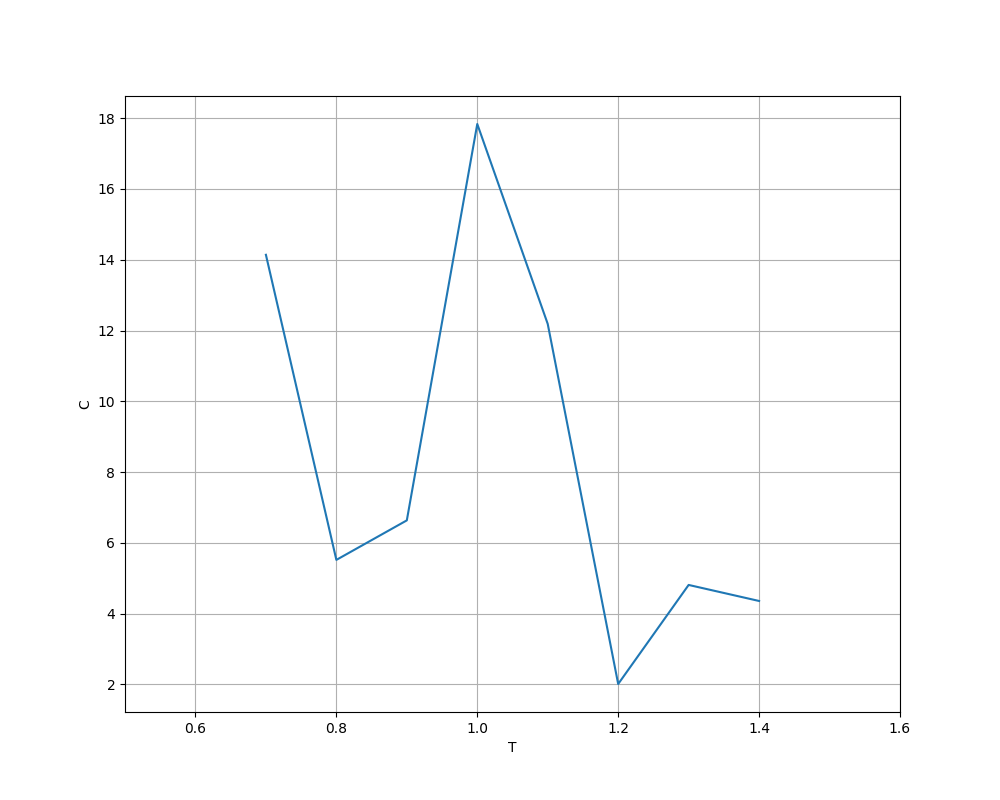
\includegraphics[width=8cm]{C_10.png}
            \caption{$10\times 10$热容$C$的温度$T$依赖}
        \end{minipage}
        \qquad
        \begin{minipage}{0.45\linewidth}
            \centering
            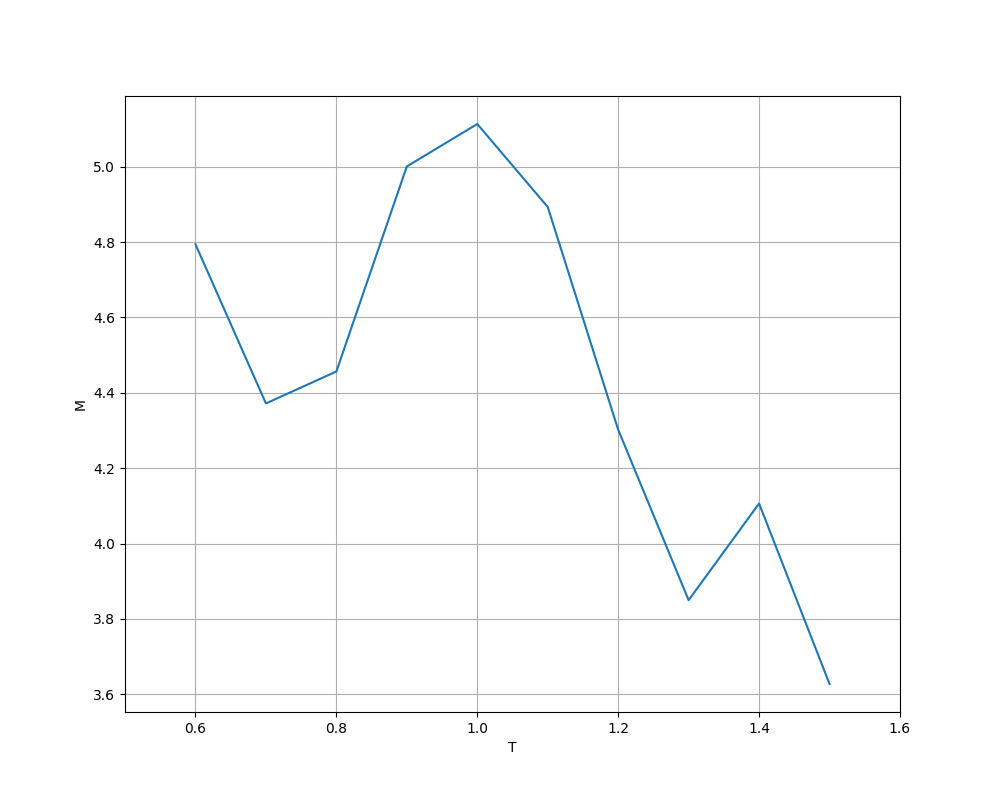
\includegraphics[width=8cm]{M_10.png}
            \caption{$10\times 10$磁化强度$M$的温度$T$依赖}
        \end{minipage}
    \end{figure}
    对于$40\times 40$格子,能量有
    \begin{figure}[H]
        \centering
        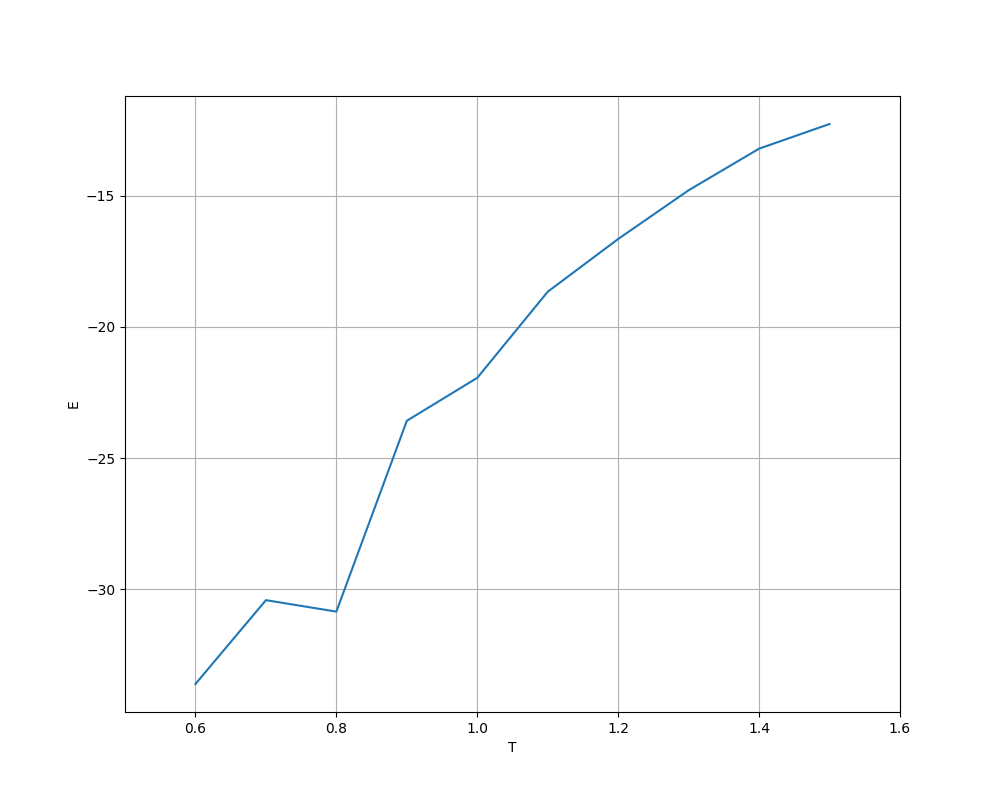
\includegraphics[width=10cm]{E_40.png}
        \caption{$40\times 40$能量$E$的温度$T$依赖}
    \end{figure}
    热容和磁化率有
    \begin{figure}[H]
        \centering
        \begin{minipage}{0.45\linewidth}
            \centering
            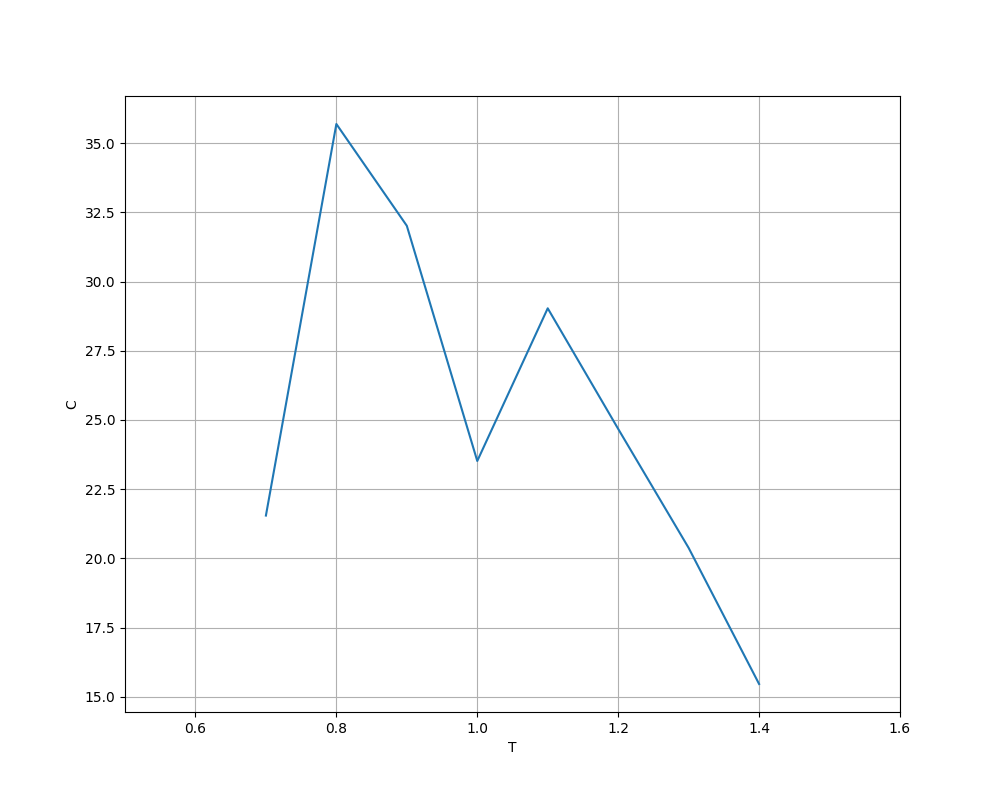
\includegraphics[width=8cm]{C_40.png}
            \caption{$40\times 40$热容$C$的温度$T$依赖}
        \end{minipage}
        \qquad
        \begin{minipage}{0.45\linewidth}
            \centering
            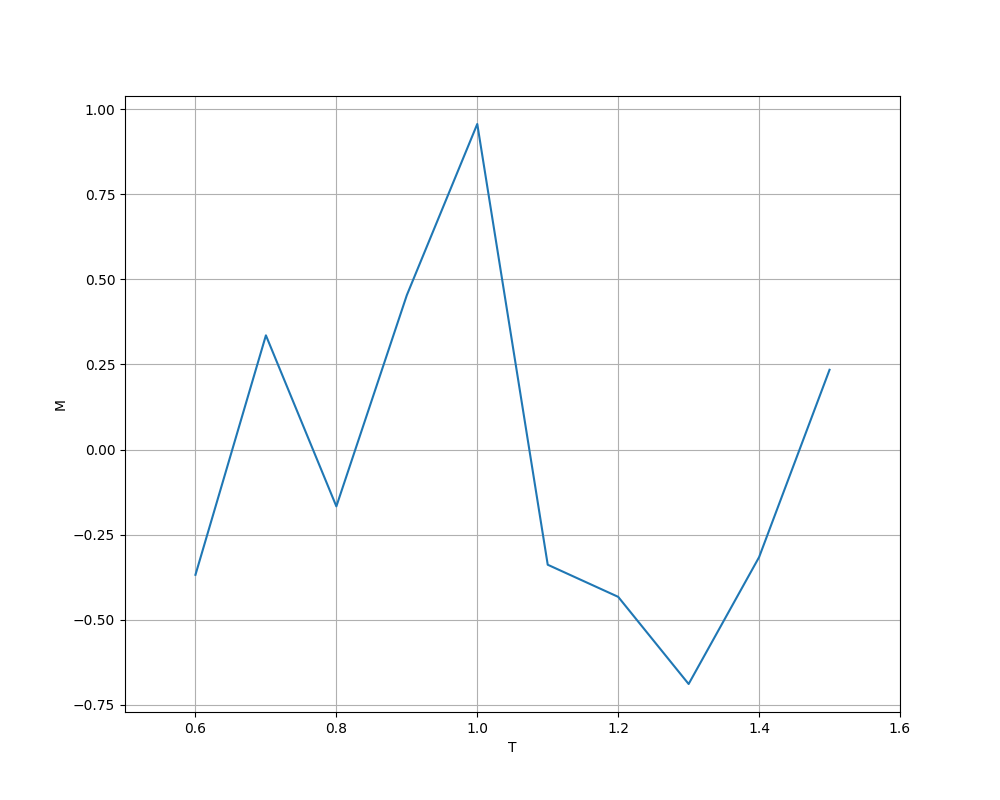
\includegraphics[width=8cm]{M_40.png}
            \caption{$40\times 40$磁化强度$M$的温度$T$依赖}
        \end{minipage}
    \end{figure}
    对于$80\times 80$格子,能量有
    \begin{figure}[H]
        \centering
        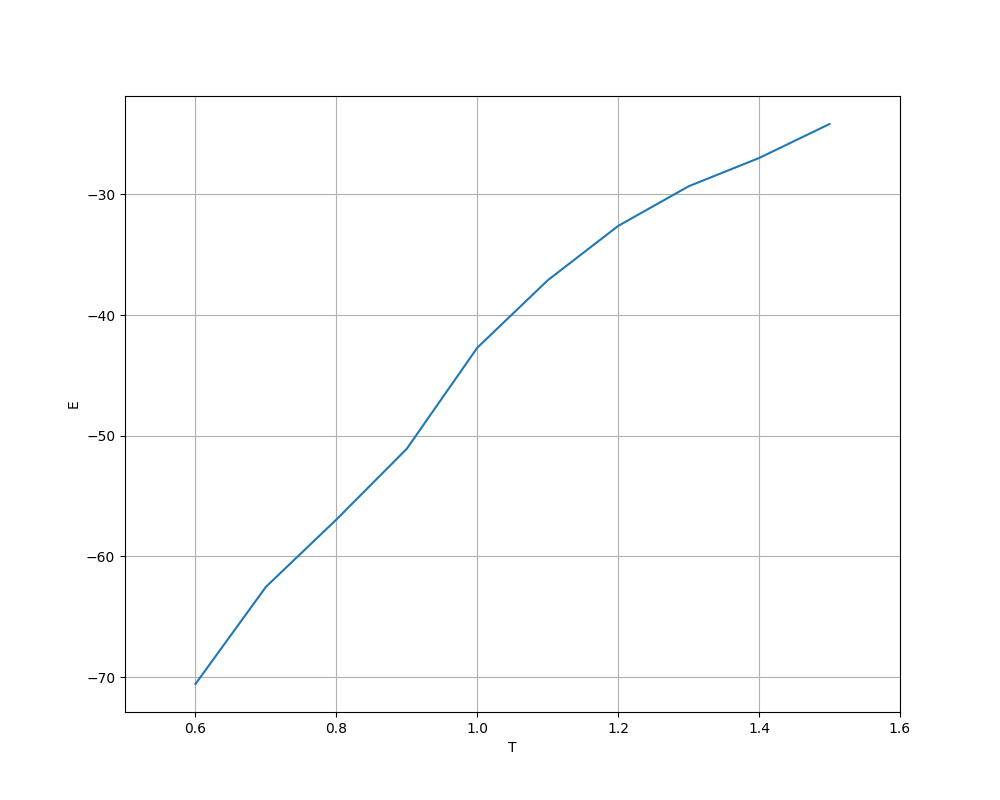
\includegraphics[width=10cm]{E_80.png}
        \caption{$80\times 80$能量$E$的温度$T$依赖}
    \end{figure}
    热容和磁化率有
    \begin{figure}[H]
        \centering
        \begin{minipage}{0.45\linewidth}
            \centering
            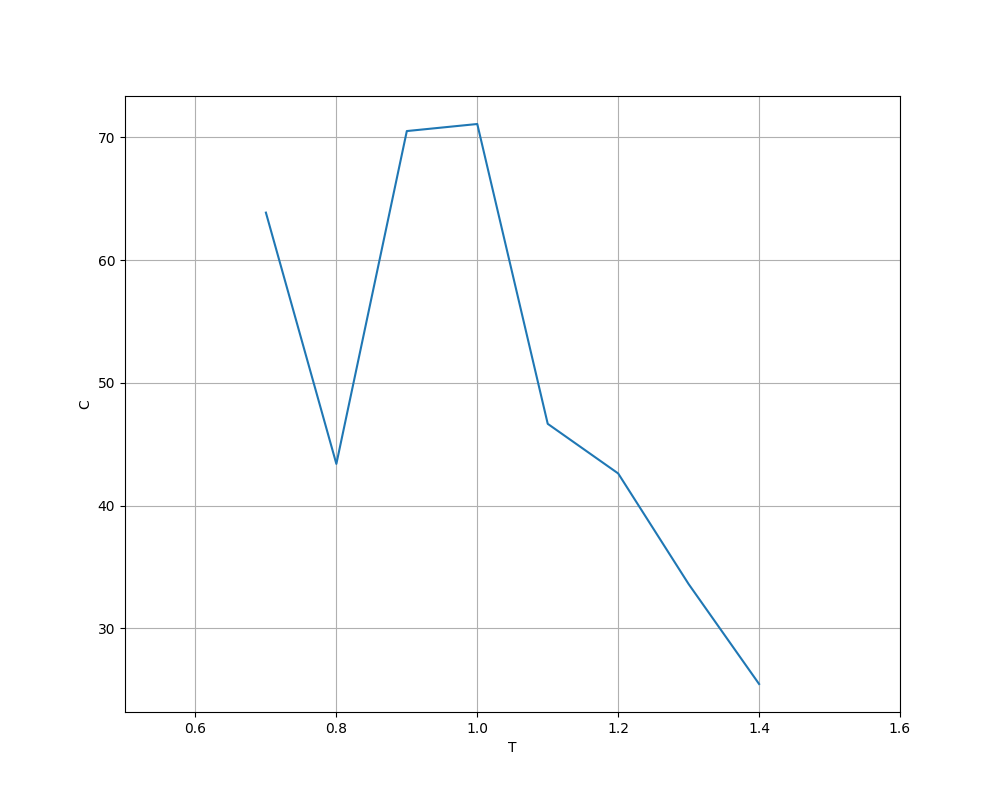
\includegraphics[width=8cm]{C_80.png}
            \caption{$80\times 80$热容$C$的温度$T$依赖}
        \end{minipage}
        \qquad
        \begin{minipage}{0.45\linewidth}
            \centering
            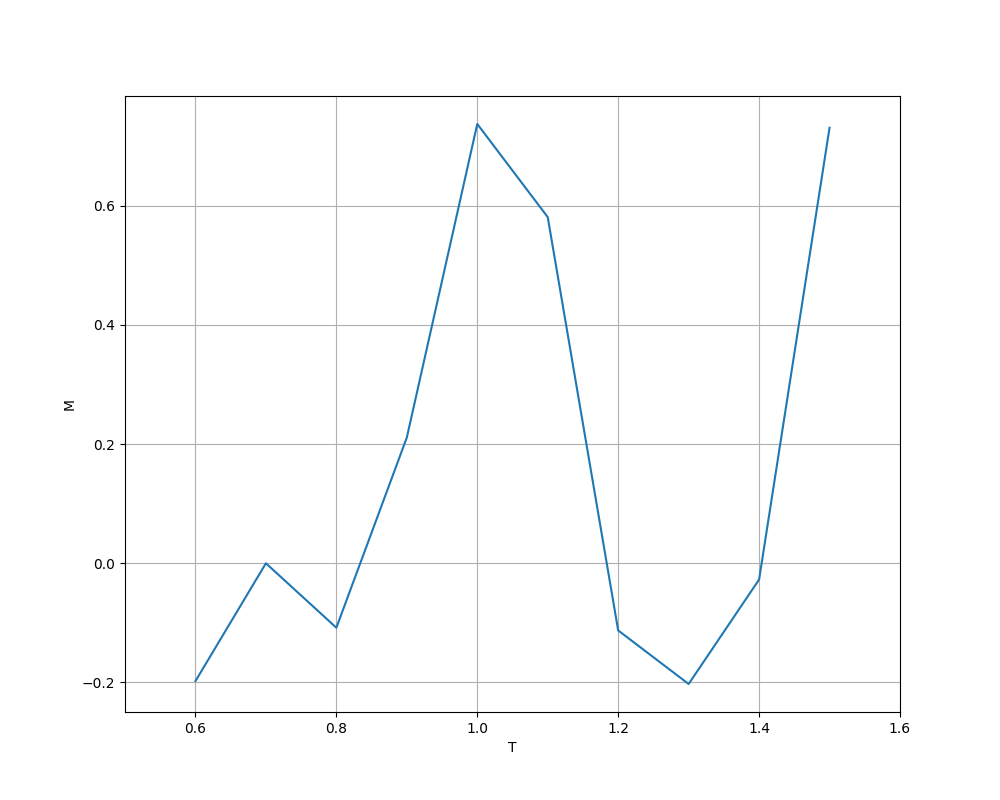
\includegraphics[width=8cm]{M_80.png}
            \caption{$80\times 80$磁化强度$M$的温度$T$依赖}
        \end{minipage}
    \end{figure}
仅有二级相变。热容$C$和磁化率$\chi$的相变在$0.8-1.4K$范围。总的来说,算法的稳定性不是很好,非常有可能是循环次数不够,时间有限,不再多算。
\end{solution}
2.2
\begin{solution}
    对于$J=1$情形的Ising模型,相当于在Potts模型上加上一个常数项,以及把Potts模型改为$J=2$。一样先粗略查看热容。蒙卡循环$10^3$次,格子大小$80\times 80$,温度范围$0.25-5K$。
借助程序“HW6计物第二题Ising热容试探.py”得到下图
    \begin{figure}[H]
        \centering
        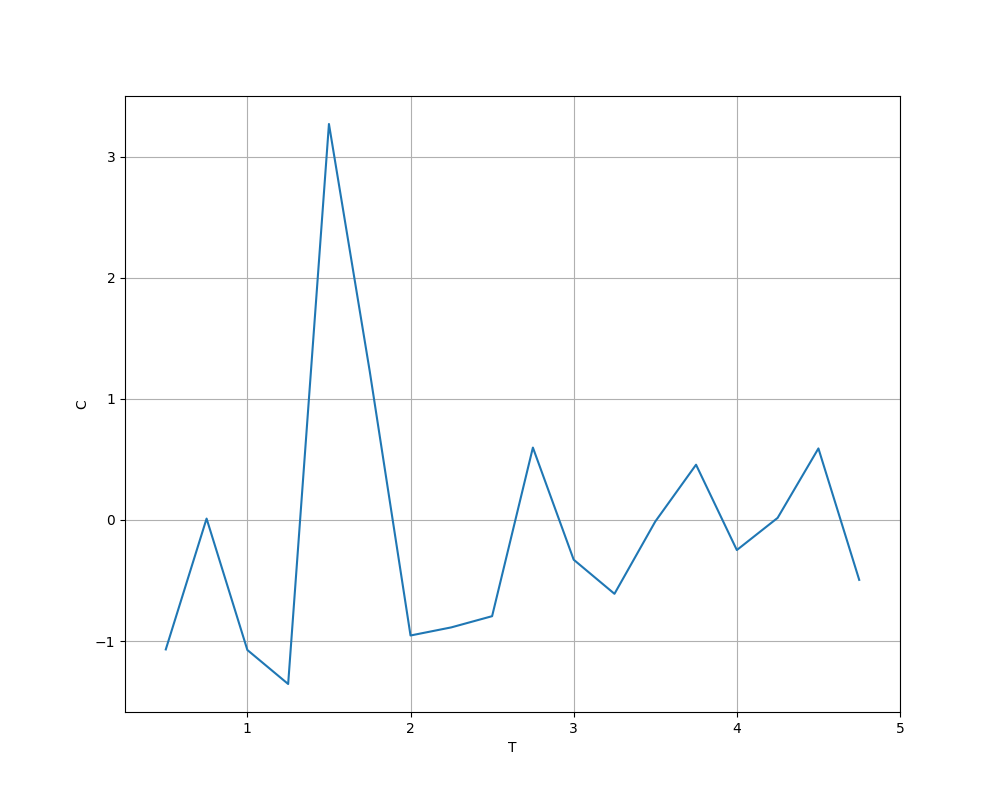
\includegraphics[width=10cm]{Ising_rough_80.png}
        \caption{Ising模型热容粗略计算}
    \end{figure}
    可以看到温度$1-3K$范围内有相变。下面仅验证$80\times 80$格子情形,Ising模型与Potts模型结论的相符程度。温度范围$1.25-3.0K$,蒙卡循环$10^5$次。
    借助程序“HW6计物第二题Ising热容.py”与“HW6计物第二题Ising磁化率.py”得到
    \begin{figure}[H]
        \centering
        \begin{minipage}{0.45\linewidth}
            \centering
            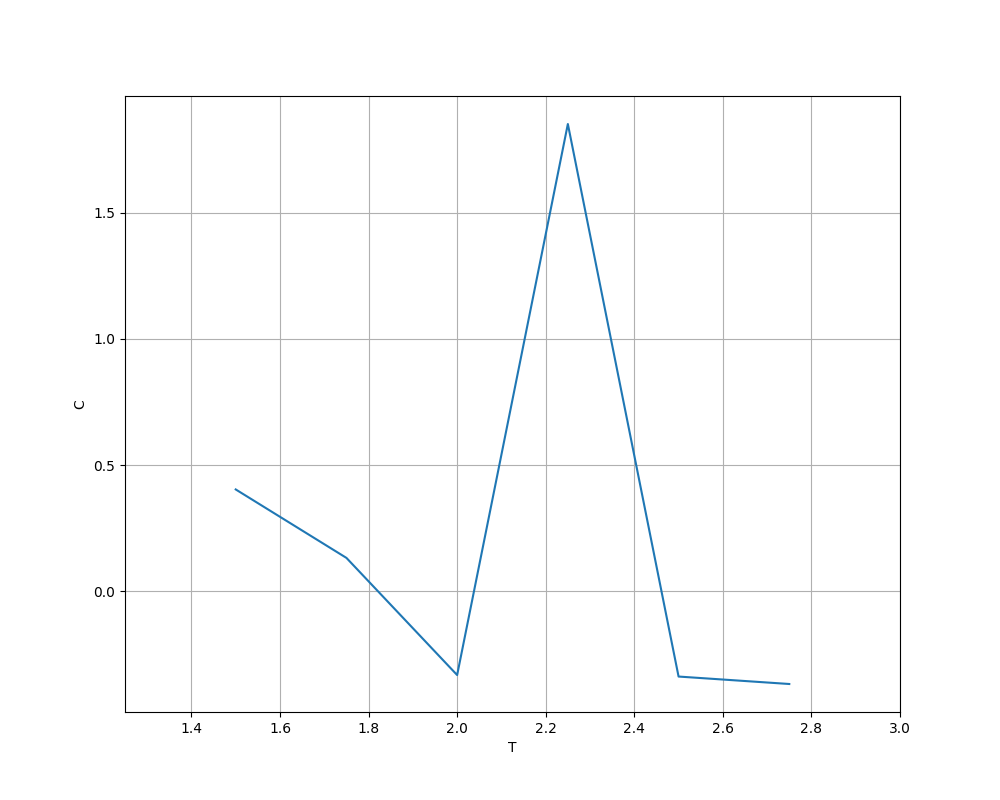
\includegraphics[width=8cm]{Ising_C_80.png}
            \caption{Ising模型$80\times 80$热容$C$的温度$T$依赖}
        \end{minipage}
        \qquad
        \begin{minipage}{0.45\linewidth}
            \centering
            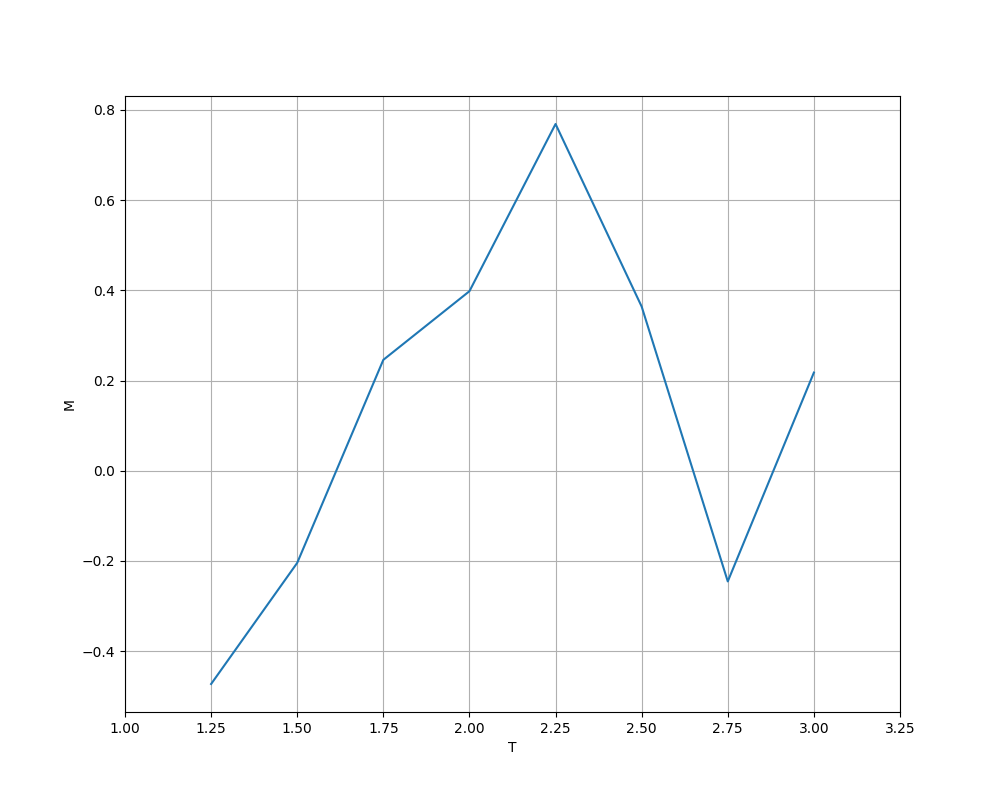
\includegraphics[width=8cm]{Ising_M_80.png}
            \caption{Ising模型$80\times 80$磁化强度$M$的温度$T$依赖}
        \end{minipage}
    \end{figure}
    可以看到热容$C$相变出现在$2-2.4K$附近,和理论精确值很像。再由程序“HW6计物第二题Ising能量.py”得到
    \begin{figure}[H]
        \centering
        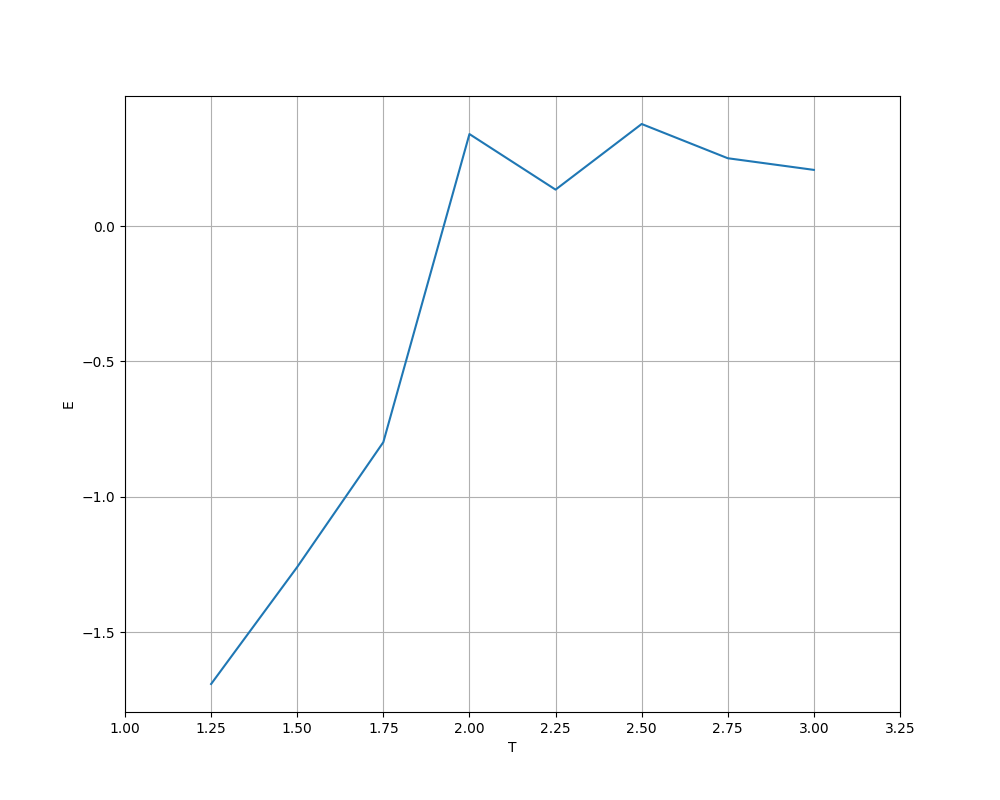
\includegraphics[width=10cm]{Ising_E_80.png}
        \caption{Ising模型$80\times 80$能量$E$的温度$T$依赖}
    \end{figure}
    故为二级相变。和Potts模型的结论相符合。

    总的来讲计算稳定性很有问题,估计是一些参数设置和循环次数的缘故。
\end{solution}
2.3
\begin{solution}
    我的算法并不需要关于$\Delta E$与$q$的表格。

    参数设置同前。对于$q=3$情形,先用热容$C$试探,借助程序“HW6计物第二题推广q3热容试探.py”得到
    \begin{figure}[H]
        \centering
        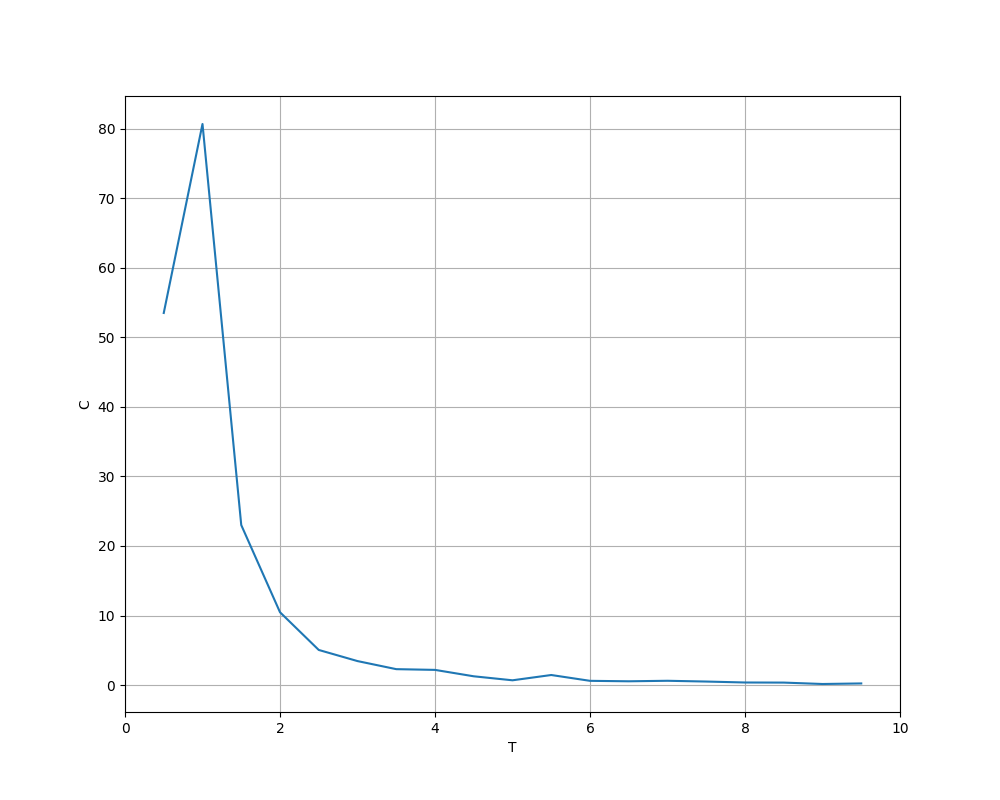
\includegraphics[width=10cm]{q3_rough.png}
        \caption{$q=3$热容$C$粗略计算}
    \end{figure}
    相变范围在$0.5-1.5K$之间。借助程序“HW6计物第二题推广q3能量.py”、“HW6计物第二题推广q3热容.py”和“HW6计物第二题推广q3磁化率.py”得到
    \begin{figure}[H]
        \centering
        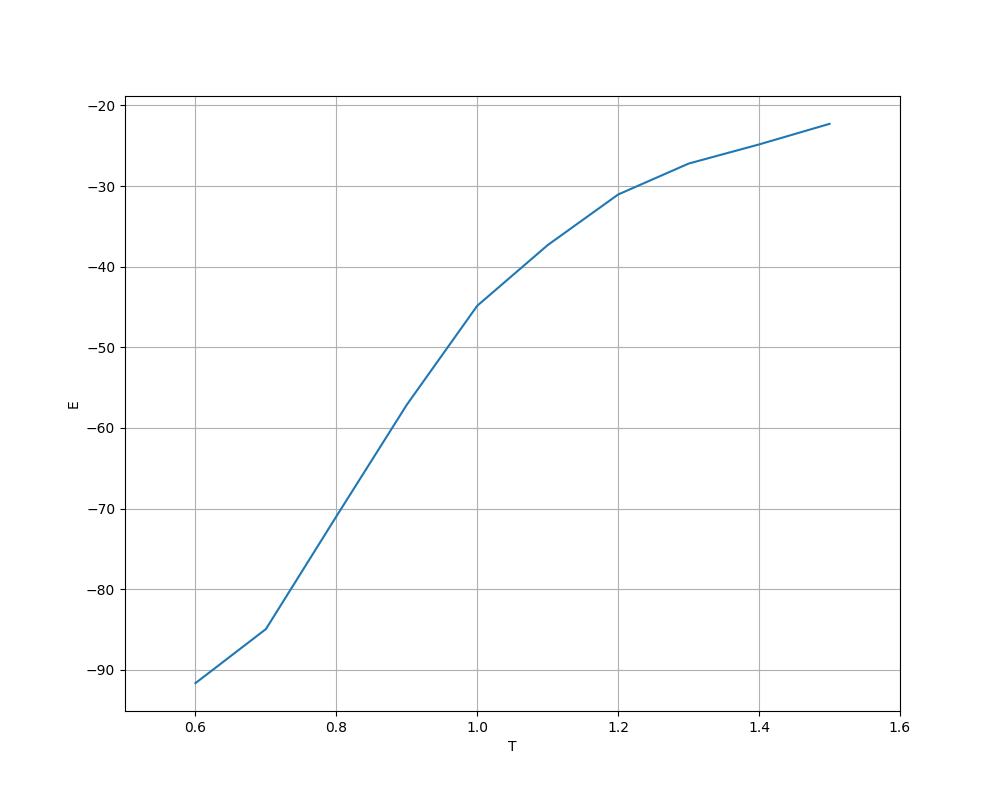
\includegraphics[width=10cm]{q3_E.png}
        \caption{$q=3$能量$E$的温度$T$依赖}
    \end{figure}
    \begin{figure}[H]
        \centering
        \begin{minipage}{0.45\linewidth}
            \centering
            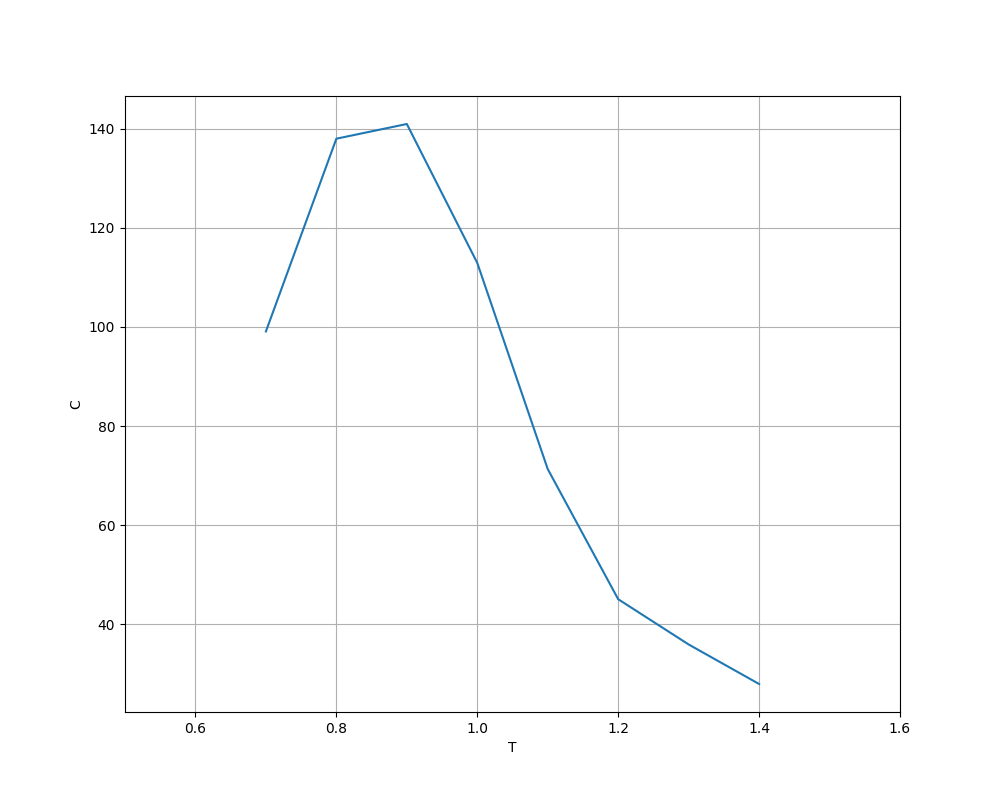
\includegraphics[width=8cm]{q3_C.png}
            \caption{$q=3$热容$C$的温度$T$依赖}
        \end{minipage}
        \qquad
        \begin{minipage}{0.45\linewidth}
            \centering
            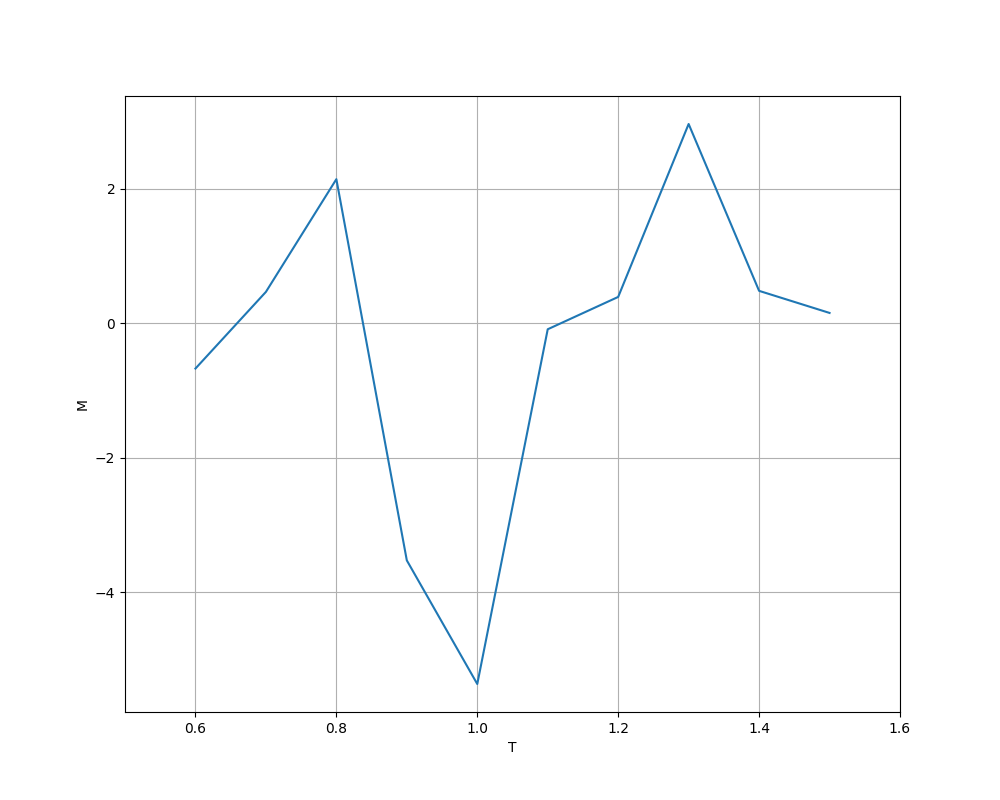
\includegraphics[width=8cm]{q3_M.png}
            \caption{$q=3$磁化强度$M$的温度$T$依赖}
        \end{minipage}
    \end{figure}
    磁化率计算的稳定性依旧不是很好。和$q=2$情形的差别不是很明显。主要关心能量$E$,再细致地计算一下
    \begin{figure}[H]
        \centering
        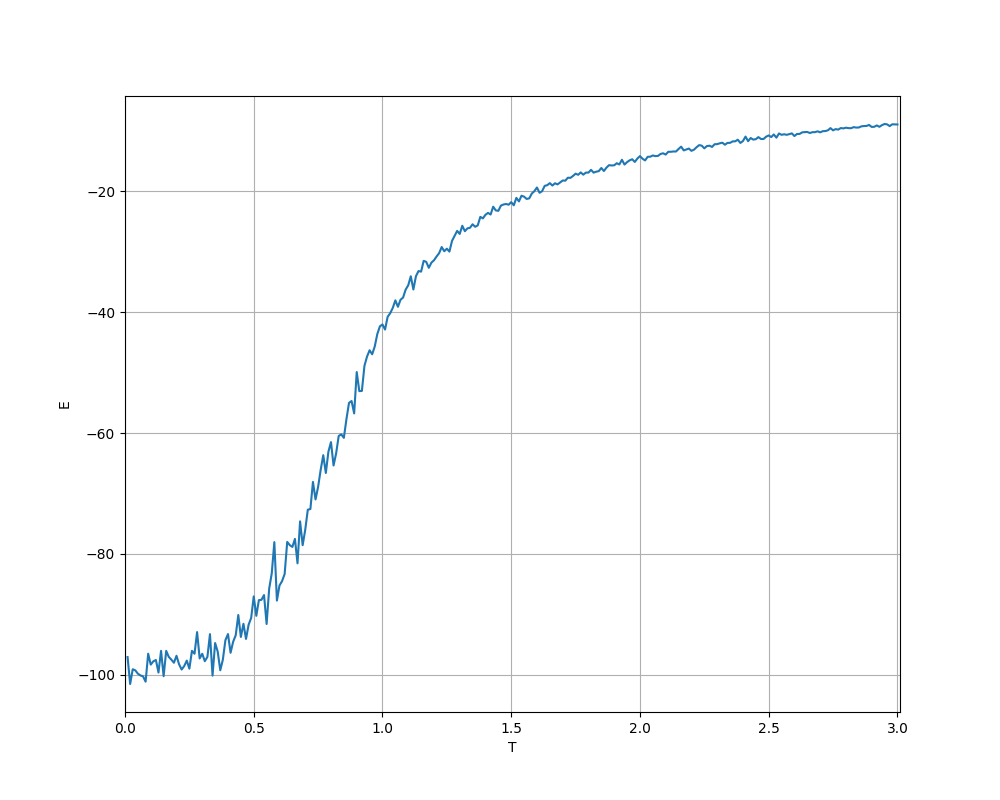
\includegraphics[width=10cm]{q3_E_.png}
        \caption{$q=3$能量$E$的温度$T$依赖}
    \end{figure}
    倾斜程度相比$q=2$情形有一些增大。

    对于$q=6$情形
    \begin{figure}[H]
        \centering
        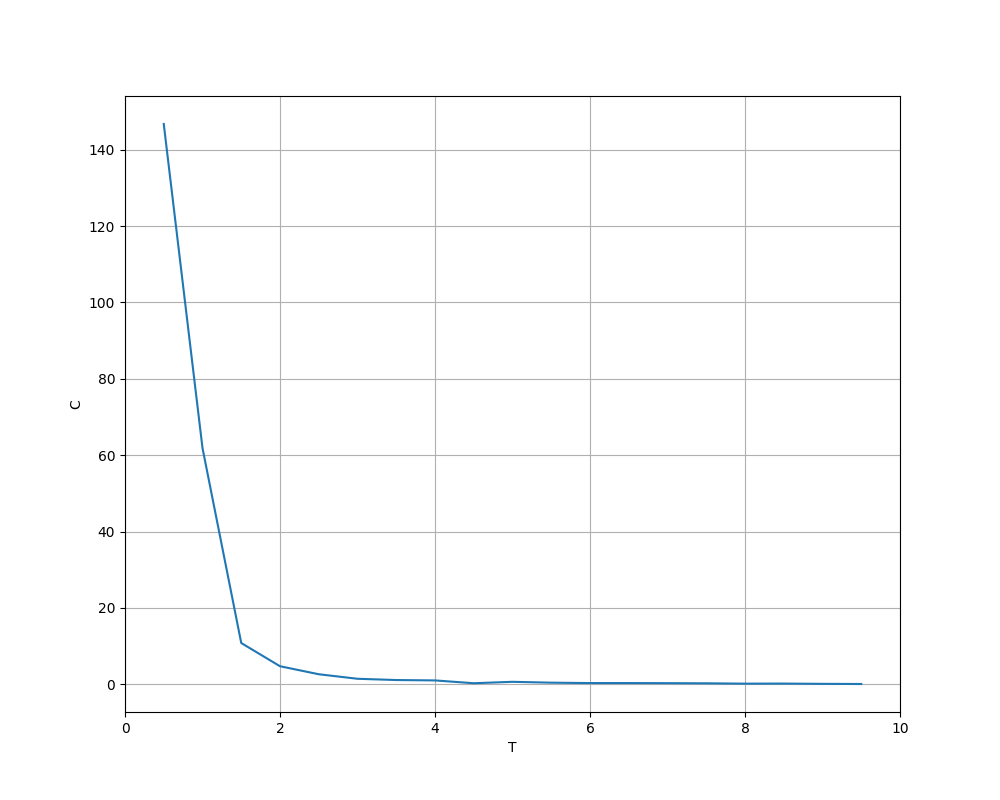
\includegraphics[width=10cm]{q6_rough.png}
        \caption{$q=6$热容$C$粗略计算}
    \end{figure}
    热容的峰值温度变得很低。能量似乎在低温有点不测。进行一些细致计算
    \begin{figure}[H]
        \centering
        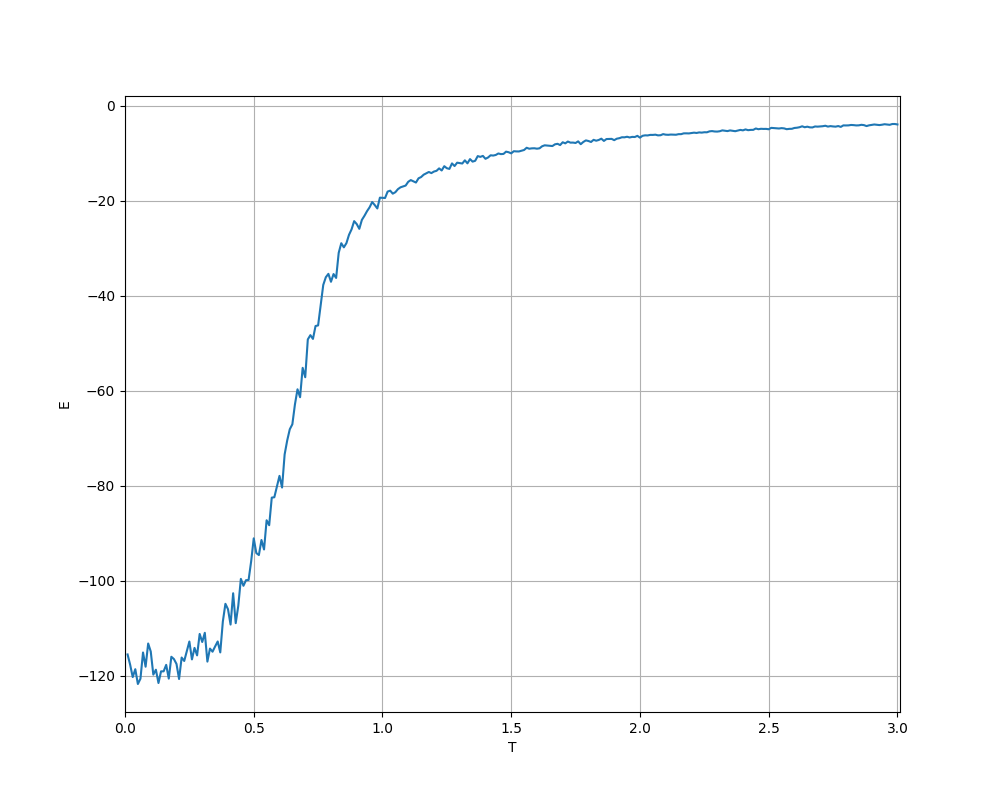
\includegraphics[width=10cm]{q6_E.png}
        \caption{$q=6$能量$E$的温度$T$依赖}
    \end{figure}
    在温度范围$0.5-1K$之间有能量的跃变,似乎出现了一级相变。
    \begin{figure}[H]
        \centering
        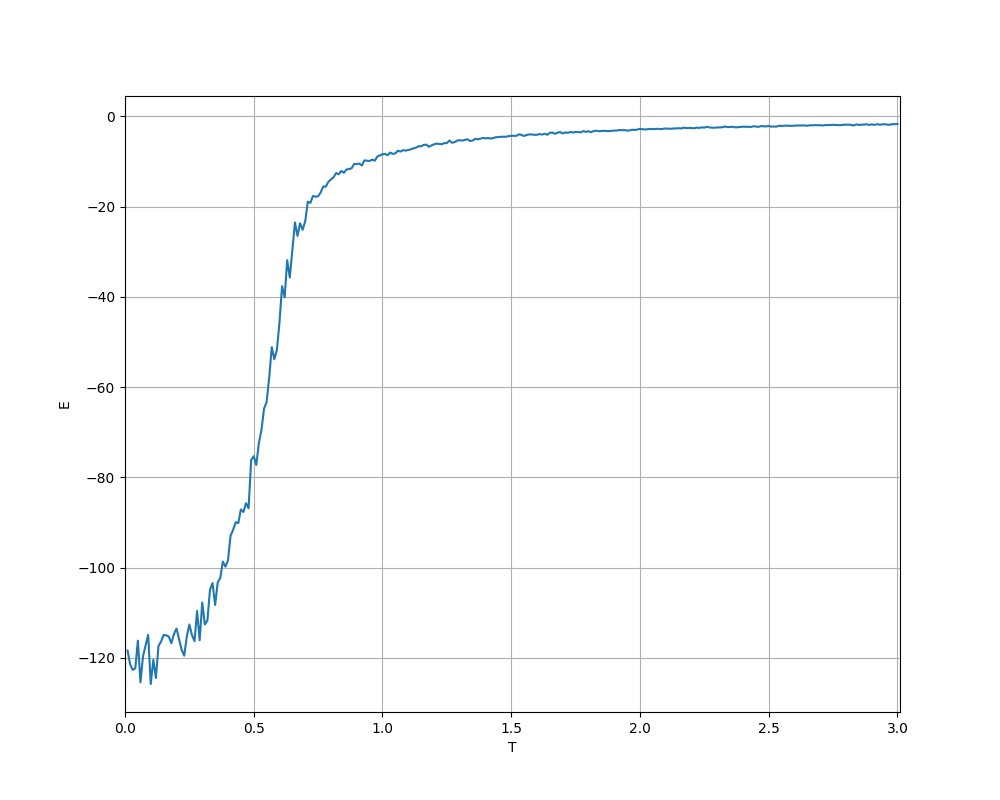
\includegraphics[width=10cm]{q10_E.png}
        \caption{$q=10$能量$E$的温度$T$依赖}
    \end{figure}
    能量跃变更明显了,是一级相变。此时热容$C$和磁导率$\chi$的计算稳定性极差,不予展示了。
\end{solution}
\end{document}